\documentclass[11pt, letterpaper]{article}
\usepackage[left=3cm, right=3cm, top=1in, bottom=20mm, includefoot, footskip=25mm]{geometry}
\usepackage[spanish, es-noshorthands]{babel}
\usepackage{hyperref}
\usepackage{graphicx}
\usepackage{csquotes}
\usepackage{fancyhdr}
\usepackage[dvipsnames, table, xcdraw]{xcolor}
\usepackage{everypage}
\usepackage{tikzpagenodes}
\usepackage{mwe}
\usepackage{fontspec}
\usepackage{booktabs}
\usetikzlibrary{calc}

\definecolor{jucuxBlue}{HTML}{011627}
%FONTS
\defaultfontfeatures{Mapping=tex-text,Scale=MatchLowercase, Color=jucuxBlue}
\setmainfont{JetBrainsMono}[Scale=1]
\setmonofont{JetBrainsMono}

% FOOTER BOX
\AddEverypageHook{
    \begin{tikzpicture}[remember picture,overlay]
        \fill[jucuxBlue] (current page.south west) rectangle (\paperwidth, -\paperheight + 57mm);
    \end{tikzpicture}
}

\begin{document}

\begin{titlepage}
	\centering
	{\bfseries \large PROPUESTA TÉCNICA\par 2IES}\\[6cm]

	
\includegraphics[width=0.4\textwidth]{assets/FUDEPLOGO.png}\\[1cm]

	\textbf{\LARGE \MakeUppercase{Sistema Informático de Seguimiento y Monitoreo Institucional}}

	\textbf{\MakeUppercase{Fundación La Paz para el Desarrollo y la Participación}}
	\vfill
	{La Paz, \today\par}
\end{titlepage}
\setlength{\baselineskip}{18pt}

% Headers and footers
\pagestyle{fancy}
\fancyhf{}
\renewcommand{\headrulewidth}{0pt}
\fancyfoot[C]{
    
\includegraphics[width=0.05\textwidth]{assets/logojucux.png}\\
    {\addfontfeature{Color=white, Scale=0.9}{\Large Jucux - \the\year}\\Empresa de desarrollo de software\\{\tiny Contáctanos vía Whatsapp: 75844266 - 79596359}}
}

\tableofcontents
\newpage
\fancyhead[R]{\thepage}
\section{Introducción y Antecedentes}

La Fundación La Paz para el Desarrollo y Participación, en cumplimiento a su objetivo de promoción del diseño y ejecución de programas y proyectos, y en base a sus esfuerzos para mantener un alto nivel de confianza y lograr el desarrollo de una mejor gestión,
solicita la implementación de un:
"SISTEMA INFORMÁTICO DE SEGUIMIENTO Y MONITOREO INSTITUCIONAL"
para sus distintos Proyectos/Programas sociales.

Este documento, elaborado por la empresa consultora 2IES, constituye así la Propuesta Técnica para la ejecución exitosa de dicho proyecto.

La propuesta se rige a los requerimientos establecidos en la novena sección , "PRESENTACIÓN DE PROPUESTAS", de los Términos de Referencia (en adelante TdR) publicados por la FUDEP en fecha 12 de noviembre de 2024 
y responde a su vez, de forma integral, a todos los demás aspectos solicitados de forma explícita o implícita en el resto de dicho documento,
presentando de modo protagónico los siguientes puntos:

\begin{itemize}
    \item Plan de Trabajo y Cronograma
    \item Metodología del proyecto
    \item Propuestas de Innovación y Valor Agregado
    \item Mockups y/o Prototipos
    \item Propuestas de Infraestructura y Arquitectura con un enfoque técnico, tecnológico, económico y práctico
    \item Propuesta de stack tecnológico
\end{itemize}

Por supuesto, lo anterior no debe verse como un aspecto limitativo a incluir otras secciones complementarias, aclaratorias y de rigor, para una propuesta técnica completa.

Para la ejecución del servicio ofertado, el contenido de este documento ha sido orientada a:

\begin{itemize}
    \item Garantizar la obtención de un producto de calidad
    \item Brindar un sistema versátil en cuanto a su utilización
    \item Establecer estructuras de datos que sean aprovechables más allá incluso de este proyecto
    \item Ofrecer interfaces amigables para el usuario final
    \item Utilizar tecnologías populares en el mercado actual
    \item Posibilitar un fácil mantenimiento del software entregado
    \item Promover el uso del software libre
    \item Anticipar posibles necesidades e inquietudes del convocante
    \item Garantizar la integridad de los datos
\end{itemize}

El  equipo de desarrollo de 2IES tiene un claro enfoque en la modernidad e innovación, pero sus valores van más allá de lo técnico por lo que se espera que la presente propuesta sea un reflejo de aquello.
%\section{Antecedentes}

La FUDEP (Fundación La Paz para el Desarrollo y la Participación) nace el año 1971 como Fundación San Gabriel consolidándose eventualmente como una institución de fomento y promoción de la participación de la población en base a los derechos humanos y el enfoque de género.

La participación de la población en distintos programas y proyectos son parte fundamental de su labor. Permitiendo beneficiar y convertir en actores relevantes a diversos participantes de la sociedad.  Incorporando a mujeres, niñas y niños en la toma de decisiones y la cogestión de proyectos.

Todo esto se refleja en su objetivo institucional que es, de acuerdo a lo expuesto en su sitio web:

\begin{displayquote}
Promover el diseño, ejecución y asesoramiento de programas, proyectos y acciones de promoción y gestión social tendientes a mejorar el nivel de vida de los destinatarios.
\end{displayquote}

Un objetivo que concuerda con su misión que expresa:

\begin{displayquote}
Somos una institución sin fines de lucro que impulsa/promueve el  empoderamiento, protagonismo y fortalezas de 
las niñas, niños, adolescentes, jóvenes y mujeres para asumir sus responsabilidades y exigir la restitución de sus derechos vulnerados.
\end{displayquote}

El pilar de los esfuerzos de la FUDEP, como podemos notar, es la gestión de programas y proyectos. Estos, al ser de tal importancia, conllevan a la aparición de ciertas necesidades, oportunidades y el claro interés de poder llevar a cabo las distintas actividades de forma transparente y que inspire confianza en todos los involucrados de tan importante misión.

\section{Problemática} % Problemática
\section{Objetivos}

A continuación se cita el objetivo general propuesto por la FUDEP y se detallan después los objetivos específicos desde un punto de vista técnico

\subsection{Objetivo General}

Implementar un sistema informático institucional autoadministrable de seguimiento y monitoreo técnico articulado al presupuestario, en base a los objetivos, resultados, indicadores y metas de proyectos//programas sociales, que permita monitorear los avances cuantitativos y cualitativos de acuerdo al marco lógico u otras herramientas de gestión de proyectos/programas, que genere información integrada, periódica, desglosada, sectorizada y otras variables de análisis de información, toma de decisiones oportunas, evaluaciones, etc.

\subsection{Objetivos Específicos}

\begin{itemize}
    \item A
\end{itemize}
%\section{Alcance del Trabajo}
\section{Enfoque Propuesto}

De acuerdo a los requerimientos analizados y en función a los objetivos se propone realizar un sistema modular con arquitectura web que no demande inicialmente un gasto excesivo en infraestructura ni en servicios de terceros, pero que, sin embargo, pueda requerirlos en cualquier momento futuro.

\subsection{Arquitectura e Infraestructura}

Inicialmente, se plantea una arquitectura monolítica, es decir, una aplicación web contenida en un solo repositorio, cumpliendo con el patrón cliente-servidor.

En cuanto a la infraestructura, existen muchas opciones, pero una de las más económicas y que bastará para las etapas iniciales con una cantidad de usuarios no mayor a los 100 activos por día es el shared hosting. Existen también varias ofertas de shared hosting, siendo la más conocida, Hostinger.

Estos servidores brindan paneles de administración intuitivos, además de precios iniciales realmente bajos, pero están limitados a ciertas tecnologías y configuraciones.

\subsection{Stack Tecnológico}

Para lograr la implementación exitosa en el menor tiempo posible, con posibilidad a mejoras futuras, escalabilidad y capacidad de funcionamiento en cualquier servidor, se propone el stack tecnológico TALL (Tailwind, Alpine, Laravel, Livewire). 

\begin{figure}[htbp]
    \centering
    
\includegraphics[width=0.7\textwidth]{assets/tall.jpg}
    \caption{Stack TALL}
    \label{fig:tall}
\end{figure}

Además, con el uso de librerías como Filament garantizamos un desarrollo eficiente y a bajos costos, además de versatilidad en caso de desear la creación de un servicio REST API a futuro para aplicaciones móviles e integraciones.

\subsection{División en módulos}

Una buena práctica es poder abstraer el sistema en módulos funcionales independientes. Nuestro análisis nos permitió identificar los siguientes:

\begin{enumerate}
\item Módulo de administración de usuarios,
\item Módulo de reservas y valoraciones (Pieza central),
\item Módulo de administración de anfitrión y registro de datos de hoteles,
\item Módulo de administración general,
\item Módulo de pagos en línea asistidos por humano
\item Módulo de pagos en línea,
\item Módulo de facturación electrónica,
\item Módulo de contabilidad básica,
\end{enumerate} % Enfoque
\section{Metodología}

A continuación se explica de manera fundamentada, sobre la base de lo descrito en este documento, la Metodología propuesta. La Metodología General que nuestra empresa, emplea y emplearía para obtener los resultados esperados, en función de los requerimientos.

\subsection{Desarrollo del Proyecto}

La metodología que seguimos, como marco de referencia, para el desarrollo de cualquier proyecto de complejidad media o alta está basada en los procesos de ciclo de ingeniería de software iterativo e incremental, desarrollado, recomendado y normalizado inicialmente por la empresa Rational Software, que hoy es propiedad de IBM, su denominación es Rational Unified Process \textquote{RUP}, 

Además, se usan principios de metodologías como SCRUM y Kanban para mejorar la comunicación con el cliente y la administración de tareas.

Tener una metodología de referencia como RUP, posibilita un profundo y razonado trabajo interdisciplinario, de equipos de profesionales que determinan los casos de uso para cada aplicación. 
Estos casos actúan como el hilo conductor a través de todas las etapas de creación del software del sistema (usando el Lenguaje de Modelado Unificado - UML), 
pues definen las acciones del usuario, los comportamientos de la aplicación y como ésta interactúa con otros programas instalados en los computadores. 
Además de especificar los casos de uso con UML, RUP nos ayuda a construir un plan de integración y evaluación del software, para brindar a los desarrolladores de Jucux y a los usuarios finales la certeza de que la totalidad del producto y cada una de sus partes se construirán como prototipos para ser evaluados y probados antes de su fase de implementación, algo que en SCRUM se llama el MVP (Minimum Viable Product). 

La metodología asegurará que obtengamos un sistema o sistemas menos susceptibles al fallo, y estables arquitectónicamente.

\begin{figure}[htbp]
    \centering
    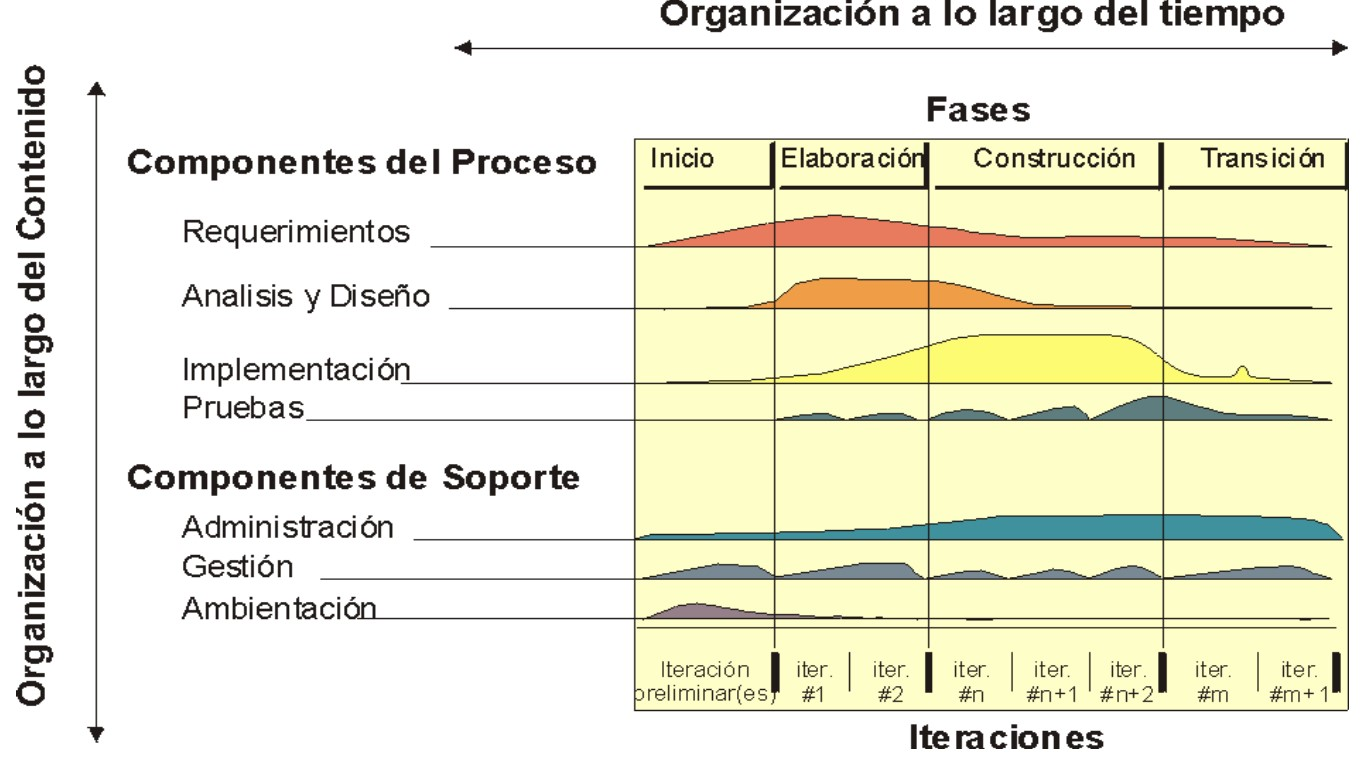
\includegraphics[width=0.7\textwidth]{assets/RUPGRAPH.JPG}
    \caption{Organización del proceso de desarrollo RUP }
    \label{fig:rupgraph}
\end{figure}

Sus características son:

\begin{itemize}
    \item Contiene las mejores prácticas de software desarrolladas por las compañías líderes de la industria.
    \item• Reduce riesgos e incrementa la predictibilidad en el desarrollo del software. • 
    \item Provee una visión y cultura estándar dentro de la organización. • 
    \item Crea y permite utilizar software reusable. • 
    \item Es soportado por herramientas muy efectivas que automatizan cada una de las fases del desarrollo del proyecto de software.
    \item Utiliza el estándar de nomenclatura Unified Modeling Language (UML).
\end{itemize}


%\section{Entregables}

A lo largo del desarrollo del proyecto, la empresa 2IES entregará los siguientes productos:

\subsection{Sistema de Seguimiento y Monitoreo Institucional}

El sistema en sí mismo contará con:
\begin{itemize}
    \item Una base de datos estructurada, con campos de auditoría
    \item Una aplicación de backend y frontend tipo web
    \item Instalación en la Infraestructura preferida por el convocante
\end{itemize}

\subsection{API para consumo de datos por parte de CMSs}

La accesibilidad de esta API dependerá de la conectividad a internet del sistema en cuestión, pero permitirá integrar en distintas plataformas la información relevante de los distintos proyectos de la fundación.

\subsection{Documentación como parte del software entregado}

Al ser un sistema web, tendrá apartados que permitirán a los usuarios de la fundación tener siempre a la mano las guías y tutoriales escritos acerca del uso del sistema.

\subsection{Guías y Tutoriales en formato multimedia disponibles vía internet}

El equipo de 2IES realizará videos sobre el uso del sistema como parte de la capacitación para que el personal de la FUDEP tenga siempre acceso oportuno a la información.

\subsection{Credenciales del sistema para garantizar confidencialidad}

Una vez concluido el proyecto, la empresa 2IES hará entrega de todas las credenciales del sistema y su infraestructura para garantizar confidencialidad y nula intervención de terceros. En adelante la responsabilidad recae sobre el convocante.


\section{Plan de Trabajo}

Un aproximado de las tareas a realizar y los tiempos que demandarán se listan a continuación:

\begin{table}[htbp]
    \centering
    \resizebox{\textwidth}{!}{%
    \begin{tabular}{@{}|l|l|@{}}
        \hline
    \rowcolor{jucuxBlue} 
    {\addfontfeature{Color=white} Etapa} & {\addfontfeature{Color=white}Tiempo Estimado}  \\ \midrule
Módulo de administración de usuarios & 20 días \\
Módulo de reservas y valoraciones (Pieza central) & 20 días \\
Módulo de administración de anfitrión y registro de datos de hoteles & 10 días \\
Módulo de administración general & 10 días \\
Módulo de pagos en línea asistidos por humano & 10 días \\
Módulo de pagos en línea & 30 días \\
Módulo de facturación electrónica & 30 días \\
Módulo de contabilidad básica & 15 días \\ \bottomrule

\end{tabular}%
    }
\end{table}

 % Plan de Trabajo

\end{document}